\documentclass[11pt]{article}
\setlength{\oddsidemargin}{.25in}
\setlength{\evensidemargin}{.25in} \setlength{\textwidth}{6in}
\setlength{\topmargin}{-0.4in} \setlength{\textheight}{8.5in}
\def\argmax{\mathop{\rm arg\,max}}

\usepackage{xspace,epsfig,amsmath,amssymb,subfig,lmodern}
\usepackage{enumerate, commath}
\usepackage{tikz, tikz-qtree}

\newtheorem{theorem}{Theorem}
\newtheorem{lemma}{Lemma}
\newtheorem{definition}{Definition}
\newtheorem{corollary}{Corollary}

\newcommand{\prob}{\ensuremath{\mathbb{P}}}

\newenvironment{sketch}{\noindent\emph{Proof Sketch:}}{$\quad \Box$}
\newenvironment{proof}{\noindent\emph{Proof:}}{$\quad \Box$}
\newenvironment{example}[2][Example]{\begin{trivlist}
\item[\hskip \labelsep {\bfseries #1}\hskip \labelsep {\bfseries #2.}]}{\end{trivlist}}
\newcommand{\handout}[5]{
   \renewcommand{\thepage}{\arabic{page}}
   \noindent
   \begin{center}
   \framebox{
      \vbox{
    \hbox to 5.78in { {\bf Choice Models in Operations}  \hfill #2
}
       \vspace{4mm}
       \hbox to 5.78in { {\Large \hfill #5  \hfill} }
       \vspace{2mm}
       \hbox to 5.78in { {\it #3 \hfill #4} }
      }
   }
   \end{center}
   \vspace*{4mm}
}

\begin{document}

\handout{}{}{Instructor: Srikanth Jagabathula}
{Scribe: Yuhang Ma} {Lecture 6: More Discussions on Model Specification}

Recall from Lecture 4, where the RUM model is introduced, we model the random utility by decomposing it into deterministic and random components, i.e.
\begin{equation*}
U_{ij} = V_{ij} + \varepsilon_{ij},
\end{equation*}
where
\begin{align*}
U_{ij}: &\text{ random utility from item $j$ of customer $i$}\\
V_{ij}: &\text{ deterministic utility from item $j$ of customer $i$}\\
\varepsilon_{ij}: &\text{ error term from item $j$ of customer $i$}
\end{align*}
The error term $\varepsilon_{ij}$ helps us to capture the differences across people when we try to model the whole population, or even if only an individual is considered, it describes some uncertainty from those unobserved features.
\section{Deterministic Component}
Let's first focus on the deterministic component $V_{ij}$. As discussed in last lecture, it can be expressed in terms of observable features as follows,
\begin{equation*}
V_{ij} = \alpha_j + \underline{\beta}^\top \underline{z}_{ij} + \underline{\gamma}_j^\top \underline{s}_i + \underline{\delta}_j^\top \underline{w}_{ij},
\end{equation*}
where
\begin{align*}
\alpha_j: &\text{ intercept term/alternative specific constant(ASC).}\\
\underline{\beta}: &\text{ generic coefficients}\\
\underline{z}_{ij}: &\text{ features that describe product $j$ at occurence $i$}\\
\underline{\gamma}_j: &\text{ alternative-specific coefficients for product $j$}\\
\underline{s}_i: &\text{ attributes that describe the occurence $i$}\\
\underline{\delta}_j: &\text{ alternative-specific coefficients for product $j$}\\
\underline{w}_{ij}: &\text{ features that describe product $j$ at occurence $i$}
\end{align*}
Notice that we \textbf{do not} model the coefficients at individual level at this point. This is because it is usually hard to collect enough information for each individual to introduce the hierarchical model, say, Mixture Logit Model. Before moving on to interpret these coefficients, let's first make some remarks on this model.
\begin{enumerate}
\item Does it make sense to introduce generic coefficients with individual-specific attributes, i.e. introducing an additional term $\underline{\eta}^\top \underline{r}_i$ as follows,
\begin{equation*}
V_{ij} = \alpha_j + \underline{\beta}^\top \underline{z}_{ij} + \underline{\gamma}_j^\top \underline{s}_i + \underline{\delta}_j^\top \underline{w}_{ij} + \underline{\eta}^\top \underline{r}_i ?
\end{equation*}

For RUM model, shifting all the utilities by the same amount \textbf{does not} affect the choice behavior. In other words, only differences in utility matter as far as choice behavior is concerned. Notice that the difference is always
\begin{equation*}
V_{ij} - V_{ij'}= (\alpha_j - \alpha_{j'}) + \underline{\beta}^\top (\underline{z}_{ij} - \underline{z}_{ij'}) + (\underline{\gamma}_j - \underline{\gamma}_{j'})^\top \underline{s}_i + (\underline{\delta}_j^\top \underline{w}_{ij} - \underline{\delta}_{j'}^\top \underline{w}_{ij'}),
\end{equation*}
regardless of the introduction of new term. Therefore, adding generic coefficients with individual-specific attributes does not result in any change in the choice behavior. 
\begin{example}[Example]1
Suppose there are two customers making choices among two products, and we observe their choice behaviors, $p_1 = \prob_1(1|\{1,2\})$ and $p_2 = \prob_2(1|\{1,2\})$ respectively. How would choice behavior of customer $1$ change, if income increased by $\$ 1$?\\ \\
To make life easier, we assume the deterministic component only depends on the income of customer $i$, $r_i$, i.e.
\begin{align*}
V_{11} = \alpha_1 + \eta r_1, && V_{21} = \alpha_1 + \eta r_2,\\
V_{12} = \alpha_2 + \eta r_1, && V_{22} = \alpha_2 + \eta r_2.
\end{align*}

If their choice behaviors follow MNL model, then 
\begin{equation*}
p_1 = p_2 = \frac{e^{\alpha_1-\alpha_2}}{1+e^{\alpha_1-\alpha_2}},
\end{equation*}
and we can directly estimate $\delta = \alpha_1 - \alpha_2$ from $p_1$, $p_2$. \\ \\
However, if given $p_1 > p_2$, then MNL model can no longer describe their choice behaviors simultaneously. Assume it still holds for each individual, and we choose item $2$ as the \textbf{reference item} by setting $V_{12} = V_{22} = \alpha_2$, then
\begin{equation*}
p_1 = \frac{e^{\alpha_1-\alpha_2+\eta r_1}}{1+e^{\alpha_1-\alpha_2+\eta r_1}} \Rightarrow \delta+\eta r_1 = \log(\frac{p_1}{1-p_1}).
\end{equation*}
Similarly, we also have
\begin{equation*}
\delta+\eta r_2 = \log(\frac{p_2}{1-p_2}).
\end{equation*}
Solve for $\delta, \eta$ using above equations, then we can compute the probability of customer $1$ purchasing item $1$ with income $r'_1$ as
\begin{equation*}
\frac{e^{\delta + \eta r'_1}}{1+e^{\delta + \eta r'_1}}.
\end{equation*}
\end{example}
\item The same logic applies to ASCs. If we include one in every item, then we cannot identify them. We can only identify their differences. Because of this, it is common to introduce ASCs and any generic coefficients with individual specific attributes in all but one \textbf{reference item}. In some applications, there may be a natural reference item, which is the no-purchase option.
\item A model with only \textbf{alternative-specific} attributes/variables is called \textbf{conditional logit model}. A model with only \textbf{individual-specific} attributes/variables is called \textbf{multinomial logit model}.
\end{enumerate}
\section{Interpretation of Coefficients}
Unlike in linear regression, the coefficients of RUM model are not directly interpretable, because cardinal value of utilities are not directly observable. We will interpret the coefficients through the impact on choice probabilities.
\begin{enumerate}[I.]
\item \textbf{Marginal effect interpretation}
\begin{enumerate}[1.]
\item \textbf{Individual/Choice-specific variables($\underline{s}_i$):}
\begin{enumerate}[(a)]
\item \textbf{Marginal effect on odds ratio:}
\vspace{0.3em}\\
\text{\quad}Suppose $\gamma_j$ is the coefficient of item $j$ corresponding to an individual-specific variable $s_i$, say, income of customer $i$. Then $e^{\gamma_j}$ captures the item's marginal impact on odds ratio of customer's choice behavior. More specifically, consider the ratio of 
\begin{equation*}
\frac{\prob(j \text{ is chosen})}{\prob(n \text{ is chosen})} = e^{V_{ij}-V_{in}}. 
\end{equation*}
We set item $n$ as the reference alternative, i.e. set $\gamma_n = 0$. If keep everything else fixed, but increase $s_i$ by $1$ unit, then the odds ratio would get multiplied by $e^{\gamma_j}$. If $\gamma_j > 0$, we can conclude the customer is more likely to buy the product.
\item \textbf{Marginal effect on purchase probability itself:}
\vspace{0.3em}\\
\text{\quad}It can be shown that under MNL model,
\begin{align*}
\frac{\partial \prob_i(j)}{\partial s_i} = \prob_i(j)\left[\gamma_j - \sum_k \prob_i(k) \gamma_k\right].
\end{align*}
We assume everything is on offer and $\prob_i(j)$ refers to the probability that customer $i$ buys product $j$. The effect of marginal increase on the choice probability depends on whether $\gamma_j$ is bigger(or smaller) relative to the average of other coefficients, i.e., $\sum_k \prob_i(k) \gamma_k$.
\end{enumerate}
\item \textbf{Alternate-specific variables($\underline{z}_{ij}$)}:
\begin{enumerate}[(a)]
\item \textbf{Marginal effect on self-elasticity:} 
\begin{align*}
\frac{\partial \prob_i(j)}{\partial z_{ij}} = \left\{ \begin{array}{ll}
        \beta\prob_i(j)[1-\prob_i(j)], & \text{ if the corresponding coefficient is generic}\\
        \delta_j\prob_i(j)[1-\prob_i(j)], & \text{ otherwise}
         \end{array} \right..
\end{align*}
The sign of coefficient determines whether the probability goes up or down. 
\item \textbf{Marginal effect on cross-elasticity:}
\begin{align*}
\frac{\partial \prob_i(j)}{\partial z_{ik}} = \left\{ \begin{array}{ll}
        -\beta\prob_i(j)\prob_i(k), & \text{ if the corresponding coefficient is generic}\\
        -\delta_k\prob_i(j)\prob_i(k), & \text{ otherwise}
         \end{array} \right..
\end{align*}
\item \textbf{Marginal effect on percentage change:}\\
\begin{align*}
\frac{\partial \log \prob_i(j)}{\partial z_{ik}} = \left\{ \begin{array}{ll}
        -\beta\prob_i(k), & \text{ if the corresponding coefficient is generic}\\
        -\delta_k\prob_i(k), & \text{ otherwise}
         \end{array} \right..
\end{align*}
That is, the percentage change in choice probability \textbf{does not} depend on product $j$. This is another implication of IIA property.
\end{enumerate}
\end{enumerate}
\item \textbf{Marginal rates of substitution}
\vspace{0.3em}\\
\text{\quad} The coefficients can also be used to explain the marginal rates of substitution among those attributes. Take a specific example as follows.
\begin{example}2
Assume $V = \alpha + \beta_1z_1 + \beta_2z_2$, say, $z_1$ is travel time in hours, $z_2$ is cost in dollars. Then $\beta_1/\beta_2$ gives us the dollar value put on an hour of travel time. To be more precise, suppose we write 
\begin{equation*}
V = \alpha + \beta_{\text{time}} \times \text{time} + \beta_{\text{cost}} \times \text{cost}. 
\end{equation*}
We expect $\beta_{\text{time}} < 0$, $\beta_{\text{cost}} < 0$. If we decrease travel time by $1$ hour, the utility of customer increases by $\abs{\beta_{\text{time}}}$, when all else is held constant. We can increase the cost by $\abs{\beta_{\text{time}}}/\abs{\beta_{\text{cost}}}$ while still not decreasing the utility. Therefore, the user is willing to pay an additional $\abs{\beta_{\text{time}}}/\abs{\beta_{\text{cost}}}$ for an hour reduction in travel time.
\end{example}
\end{enumerate}
\section{Error Term}
As of now, we all concentrate on the deterministic component $V_{ij}$ in the model. Let's turn to discussing about the error term $\varepsilon_{ij}$ a little bit. The MNL model assumes that the error terms are independent across the items and individuals. The problem with this assumption is that it requires \textbf{all} the unobservables to be independent across both items and individuals. However, it does not always hold in rea
\begin{example}[Example] 3
We have $4$ options, car, carpool, bus and train. We observe travel time($t$) and travel cost($c$) for each mode of transportation and use the following model,
\begin{align*}
V_{\text{car}} &= \beta_t \times t_{\text{car}} + \beta_c \times c_{\text{car}} + \varepsilon_{\text{car}}\\
V_{\text{carpool}} &= \beta_t \times t_{\text{carpool}} + \beta_c \times c_{\text{carpool}} + \varepsilon_{\text{carpool}}\\
V_{\text{bus}} &= \beta_t \times t_{\text{bus}} + \beta_c \times c_{\text{bus}} + \varepsilon_{\text{bus}}\\
V_{\text{train}} &= \beta_t \times t_{\text{train}} + \beta_c \times c_{\text{train}} + \varepsilon_{\text{train}}
\end{align*}
However, there could be correlations among $\varepsilon$'s across the \textbf{items}, for instance, customer who dislike public transportation will sample small(or even negative) utility for both bus and train. Additionally there could also be correlations among unobervables across the \textbf{individuals} as well. 
\end{example}
We tackle this using either a \textbf{Nested Logit(NL) Model} or \textbf{Mixture Logit(ML) Model}. NL is used to capture the correlation in unobservables across the \textbf{items} and ML is used to capture the correlation in unobservables across \textbf{individuals}. Think of the above example, we can model it under an NL model as in Figure \ref{fig:1}. The products in the same nest share some similarities and so that there probably are correlated between unobserved features.
\begin{figure}[!ht]
\begin{center}
\begin{tikzpicture}[grow'=down]
\Tree [.root [.{nest $2$} train bus ] [.{nest $1$} carpool car ] ]
\end{tikzpicture}
\end{center}
\caption{The Nested Logit Model for Example 3}\label{fig:1}
\end{figure}
\section{Nested Logit Model}
Although it can be generalized to $d$-level nested logit model, we focus on a $2$-level one right now. Assume that products are partitioned into $m$ nests. Each item belongs to \textbf{exactly one} nest. Each nest contains $n$ items. Total number of products is $mn$.(We can also generalize it to the case where there are different number of products across the nests.) For each item $j$ in nest $\ell$, we model its random utility as following,
\begin{align*}
U_{\ell j} = W_\ell + Y_{\ell j} + \tilde{\varepsilon}_\ell + \tilde{\varepsilon}_{\ell j},
\end{align*}
where
\begin{align*}
U_{\ell j}: &\text{ random utility of product $j$ in nest $\ell$}\\
W_\ell: &\text{ nest-specific utility for nest $\ell$}\\
Y_{\ell j}: &\text{ utility from item $j$ in nest $\ell$}\\
\tilde{\varepsilon}_\ell: &\text{ nest-specific unobserved utility for nest $\ell$(introduces correlation)}\\
\tilde{\varepsilon}_{\ell j}: &\text{ unobserved utility from item $j$ in nest $\ell$}
\end{align*}
Then we have the following assumption for those error terms.\\ \\
\textbf{Assumptions:}
\begin{enumerate}[1.]
\item $\tilde{\varepsilon}_\ell$, $\tilde{\varepsilon}_{\ell j}$ are independent across nests and products within nests.
\item $\tilde{\varepsilon}_{\ell j}$ are independent identically distributed Gumbel(0, $\mu_\ell$), $\mu_\ell > 0$.
\item $\tilde{\varepsilon}_\ell$ are distributed such that $\max_{j \in S_\ell} U_{j \ell}$ is Gumbel with scale $\lambda_\ell > 0$, for all the subsets of items $S_\ell$ in nest $\ell$.
\end{enumerate}
To better understand where the third assumption comes from, suppose we partition the four products as in Figure \ref{fig:2}.
\begin{figure}[!ht]
\begin{center}
\begin{tikzpicture}[grow'=down]
\Tree [.root [.{nest $2$} 4 3 ] [.{nest $1$} 2 1 ] ]
\end{tikzpicture}
\end{center}
\caption{The Nested Logit Model for Example 4}\label{fig:2}
\end{figure}
\begin{example}[Example] 4
Under the NL model in Figure \ref{fig:2}, the random utilities of four items can be modeled as
\begin{align*}
U_{11} = V_{11} + \tilde{\varepsilon}_1 + \tilde{\varepsilon}_{11}, && U_{12} = V_{12} + \tilde{\varepsilon}_1 + \tilde{\varepsilon}_{12},\\
U_{23} = V_{23} + \tilde{\varepsilon}_2 + \tilde{\varepsilon}_{23}, && U_{24} = V_{24} + \tilde{\varepsilon}_2 + \tilde{\varepsilon}_{24}.
\end{align*}
In Assumption 3, we want
\begin{align*}
\max\{U_{11}, U_{12}\} &= \max \{V_{11} + \tilde{\varepsilon}_1 + \tilde{\varepsilon}_{11}, V_{12} + \tilde{\varepsilon}_1 + \tilde{\varepsilon}_{12}\}\\
&= \tilde{\varepsilon}_1 + \max \{V_{11} + \tilde{\varepsilon}_{11}, V_{12} + \tilde{\varepsilon}_{12}\}\\
&= \tilde{\varepsilon}_1 + \text{Gumbel}(\underline{\quad}, \mu_\ell) \overset{d}\sim\text{Gumbel}(\underline{\quad}, \lambda_\ell).
\end{align*}
\end{example}
More generally, denote $\prob(j\ell) = \prob(j \text{ from nest $\ell$ is chosen})$, $\prob(\ell) = \prob(\text{an item from nest $\ell$ is chosen})$, $\prob(j|\ell) = \prob(j \text{ is chosen}|\text{ item from nest $\ell$ is chosen})$. Thus,
\begin{align*}
\prob(j \ell) = \prob(\ell) \times \prob(j|\ell),
\end{align*}
where
\begin{align*}
\prob(\ell) &= \prob(\max_{j \in N_\ell} U_{\ell j} \geq \max_{j \in N_{\ell'}} U_{\ell' j}, \forall \ell' \neq \ell)\\
&= \prob(W_\ell + \tilde{\varepsilon}_\ell + \max_{j \in N_\ell}(Y_{\ell j} + \tilde{\varepsilon}_{\ell j}) \geq W_{\ell'} + \tilde{\varepsilon}_{\ell'} + \max_{j \in N_{\ell'}}(Y_{\ell' j} + \tilde{\varepsilon}_{\ell' j}), \forall \ell' \neq \ell)
\end{align*}
Let $\max_{j \in N_\ell}(Y_{\ell j} + \tilde{\varepsilon}_{\ell j}) = \frac{1}{\mu_\ell} IV_\ell + \varepsilon_\ell$, where $\varepsilon_\ell \overset{d}\sim$ Gumbel($0, \mu_\ell$) and $IV_\ell = \log(\sum_{j \in N_\ell} e^{\mu_\ell Y_{\ell j}})$, where $IV_\ell$ is called the inclusive value/utility of nest $\ell$, then
\begin{align*}
\prob(\ell) &= \prob(W_\ell + \frac{1}{\mu_\ell} IV_\ell +\tilde{\varepsilon}_\ell + \varepsilon_\ell \geq W_{\ell'} + \frac{1}{\mu_{\ell'}} IV_{\ell'} +\tilde{\varepsilon}_{\ell'} + \varepsilon_{\ell'}, \forall \ell' \neq \ell)
\end{align*}
We want $\tilde{\varepsilon}_\ell + \varepsilon_\ell$ to be independent and Gumbel of same scale to utilize the formula from MNL model and thus we assume that $\tilde{\varepsilon}_\ell + \varepsilon_\ell \overset{d}\sim$ Gumbel($0, \lambda_\ell$), which is exactly the third assumption we made for NL model. Then by formula for the MNL,
\begin{equation*}
\prob(\ell) = \frac{e^{\lambda_\ell(W_\ell + \frac{1}{\mu_\ell}IV_\ell)}}{\sum_{\ell'}e^{\lambda_{\ell'}(W_{\ell'} + \frac{1}{\mu_{\ell'}}IV_{\ell'})}}.
\end{equation*}
\end{document}
